\section{Individuelle Richtlinien für jedes der Labore}

Der Lehrstuhl für Medieninformatik verfügt über drei Labore: Das \emph{Future Interaction Lab} (FIL) im Gebäude PT3, den Eyetracking-Classroom im Sammelgebäude und Versuchsraum 4 (VR4) in der TechBase.

\medskip
\noindent
Das FIL ist mit Trennwänden ausgestattet, die bei Bedarf geöffnet werden können, ist aber normalerweise in drei einzelne Räume mit eigenen Eingangstüren aufgeteilt.
Alle Räume sind an eine Lüftungsanlage angeschlossen, die die Raumluft nach Außen umwälzt.
Das Usability-Labor und die Werkstatt verfügen über keine weiteren Lüftungsmöglichkeiten.
Im Besprechungsraum befindet sich ein Fenster, über das zusätzlich gelüftet werden kann.
Alle Räume verfügen über einen separaten Zugang zum Gang. 

\medskip
\begin{figure}[h!]
\centering
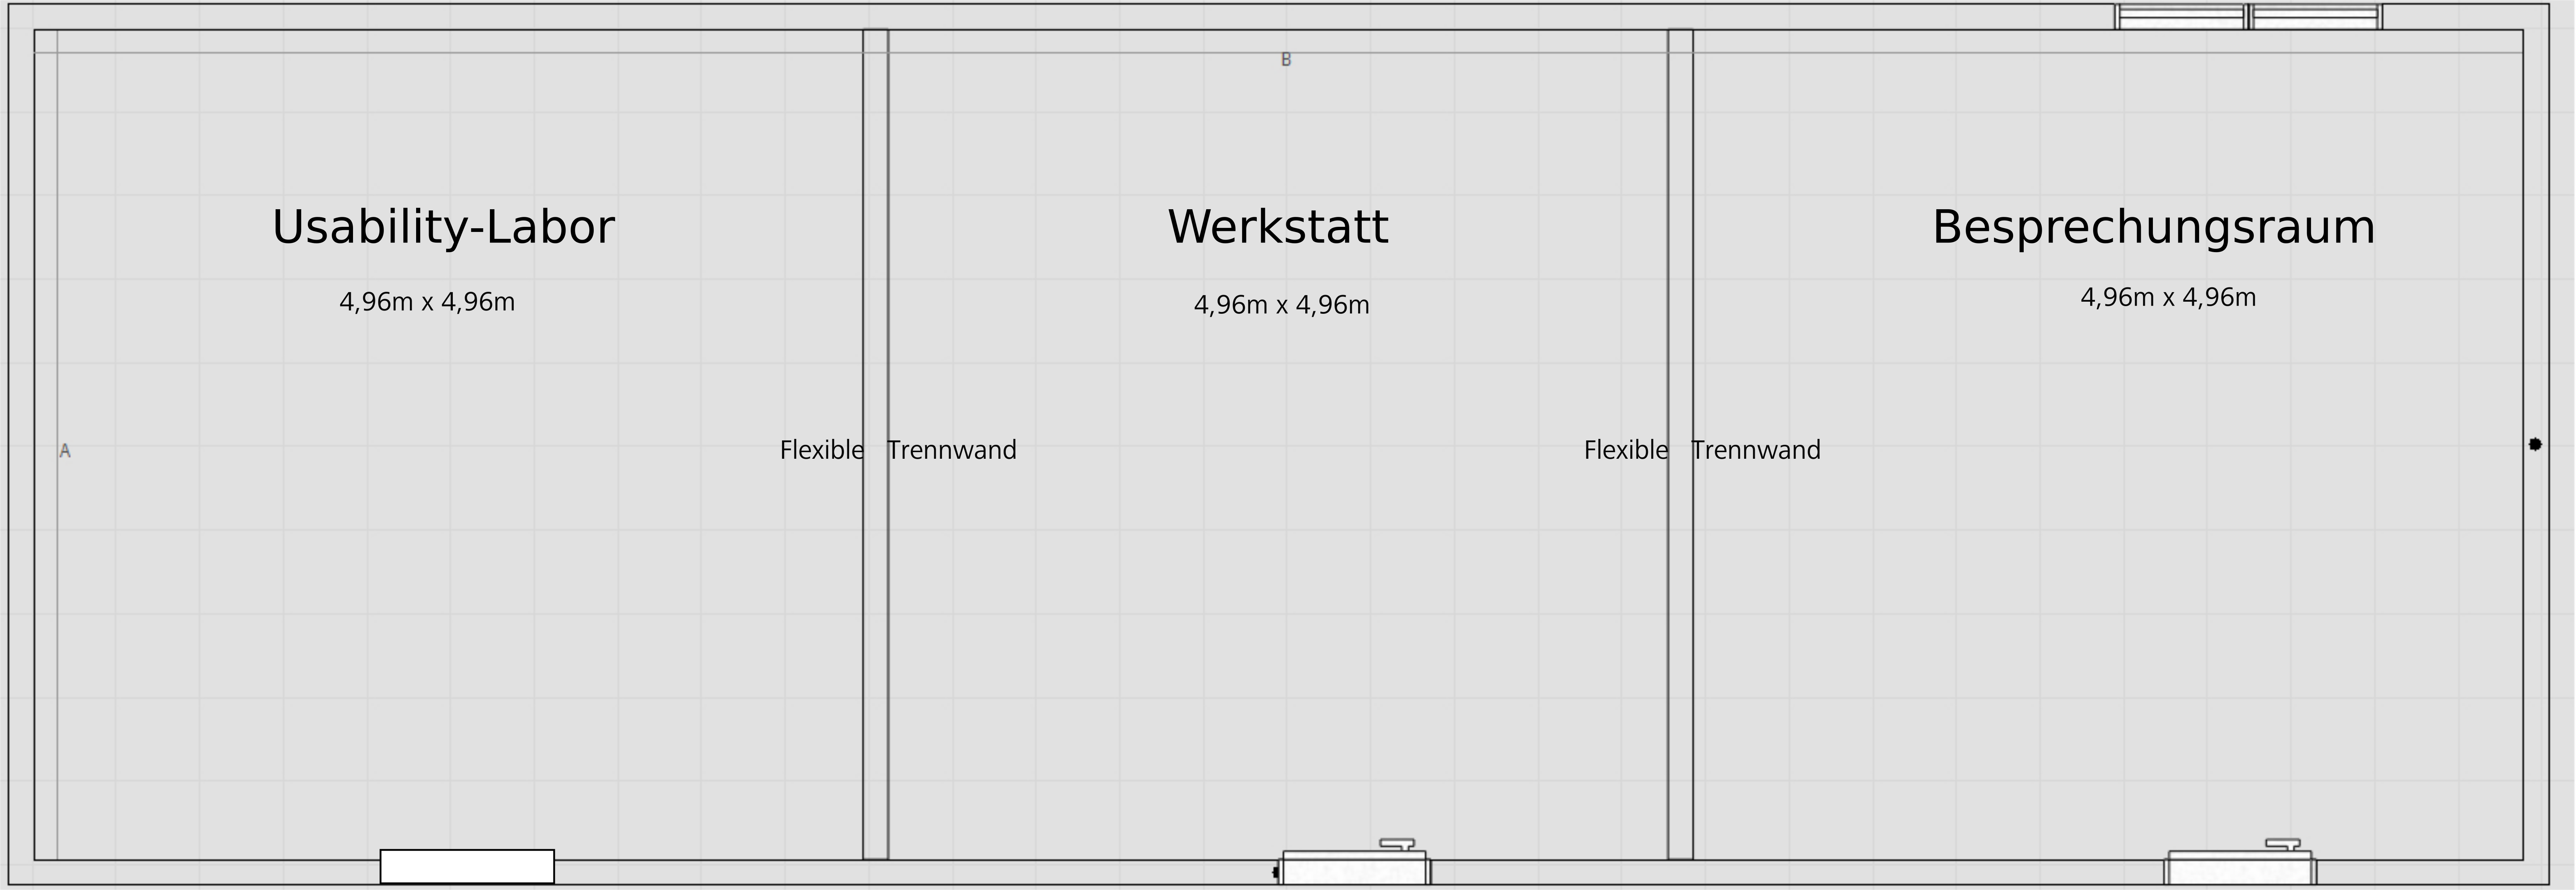
\includegraphics[width=0.7\textwidth]{../raumpläne/fil}
\end{figure}

\medskip
\noindent
VR4 ist in drei Bereiche aufgeteilt, jedoch muss der Hauptraum (VR4 Labor) durchquert werden um in die anderen beiden Bereiche (VR4 Studio und VR4 Werkstatt) zu gelangen.
Da sich VR4 nicht im Universitätsgebäude sondern in der TechBase befindet, wurde zusätzlich mit deren Hausverwaltung geklärt, dass auch Studierende und Proband*Innen das Gebäude betreten dürfen.

\medskip
\begin{figure}[h!]
\centering
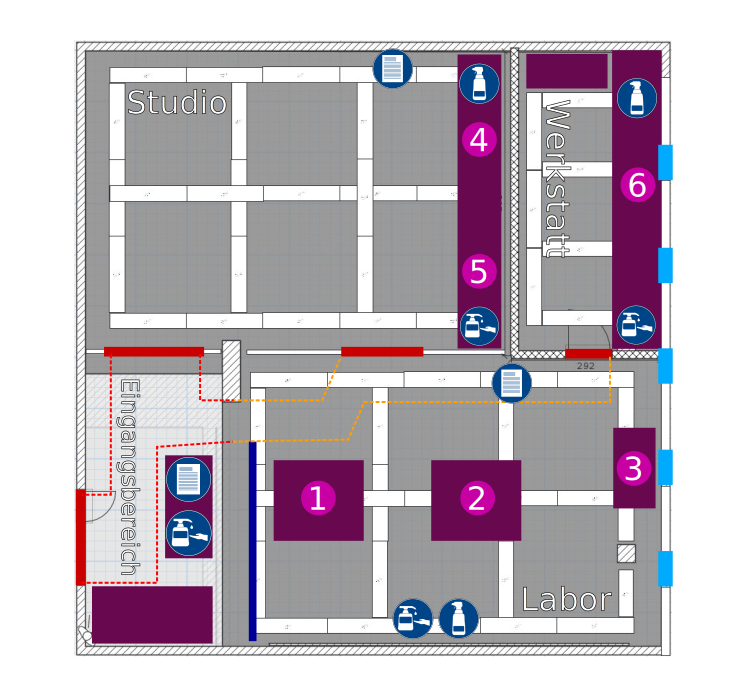
\includegraphics[width=0.5\textwidth]{../raumpläne/vr4}
\end{figure}

\medskip
\noindent
Der Eye-Tracking-Classroom besteht aus einem Laborbereich, einem ehemaligen CIP-Pool, sowie einem Beobachtungs- und Entwicklungsbereich.
Beide Räume verfügen über separate Zugänge über den Gang und sind durch eine Zwischentür miteinander verbunden.
Die Belüftung erfolgt über die Fenster, die in jedem der Räume vorhanden sind:

\medskip
\begin{figure}[h!]
\centering
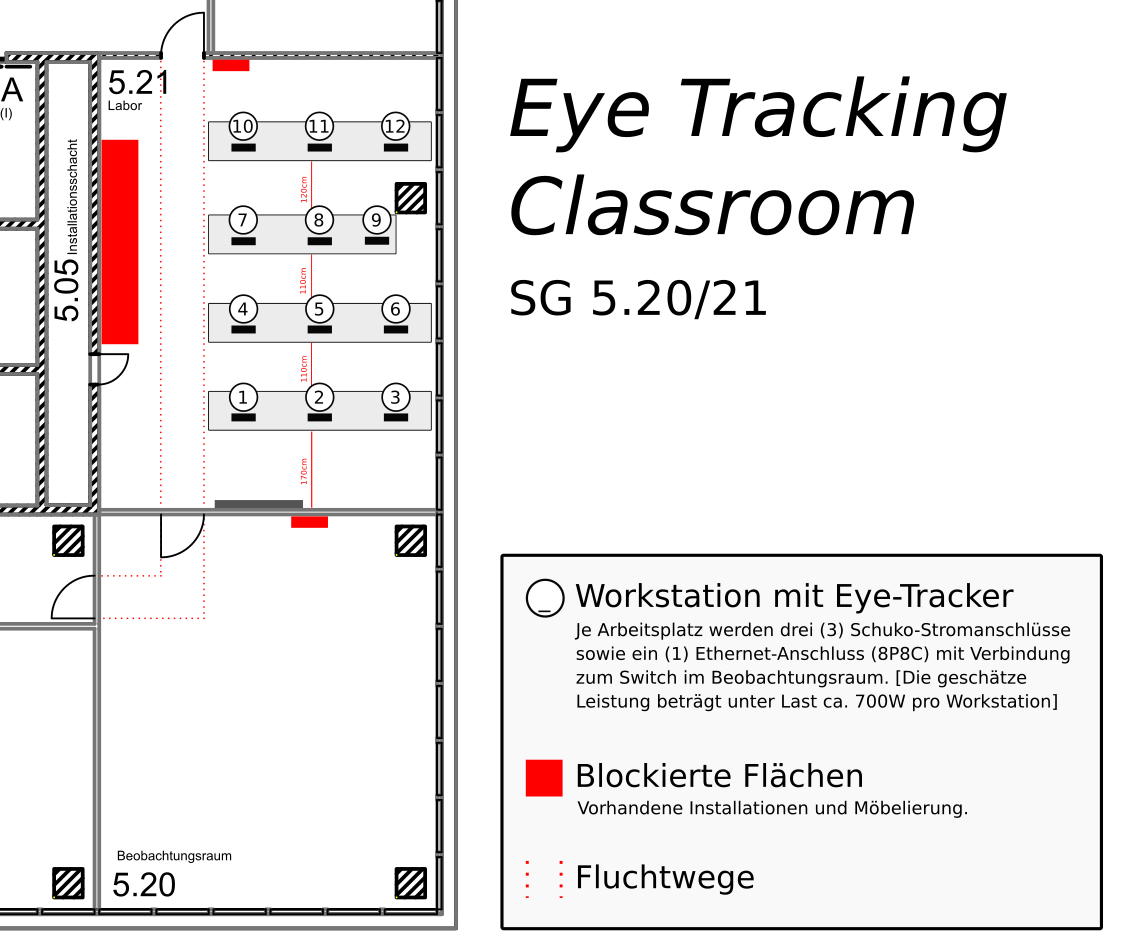
\includegraphics[width=0.5\textwidth]{../raumpläne/eyetracking-classroom}
\end{figure}

\medskip
\noindent
Im Folgenden werden die Art der Nutzung während der Einschränkungen, sowie die praktische Umsetzung der Hyginemaßnahmen für jeden der Räume dargestellt.

\subsection{Future Interaction Lab: Usability-Labor}

\labinfo{Klassische Benutzerstudie, Entwicklungsarbeiten, Medienproduktion}{1}{Alexander Bazo, Christoph Härtl}

\noindent
Das Usability-Labor dient vorrangig der Durchführung von Nutzerstudien, insbesondere solcher Experimente, die eine “Alltagssituation” als Testumgebung erfordern.
Dazu sind neben einem klassischen Arbeitsplatz auch ein Sofa und Fernseher vorhanden.
Der Arbeitsplatz kann zusätzlich auch für Entwicklungsarbeiten und die Medienproduktion eingesetzt werden.
Bei Verwendung der vorhandenen Geräte (Workstations) muss nach Gebrauch eine Desinfektion der Eingabegeräte (Maus \& Tastatur) erfolgen.

\medskip
\noindent
Bei Verwendung des Raums für die Durchführung von Nutzerstudien wird die Fläche  durch Öffnen der Trennwand zu der angrenzenden Werkstatt erweitert.
Damit ist dann auch eine Trennung von Ein- und Ausgängen für die Testpersonen möglich.
Die räumlichen und einrichtungstechnischen  Beschränkungen im Labor schließen Studien mit mehr als einem Probanden aus.
Insgesamt sollten im Raum nicht mehr als zwei Personen (ProbandIn und TestleiterIn) anwesend sein.
Denkbar sind zusätzliche BeobachterIn in einem der angrenzenden Räume.
Entsprechende Videotechnik steht im Labor zur Verfügung.

\subsection{Future Interaction Lab: Werkstatt}

\labinfo{Entwicklungsarbeiten, Medienproduktion}{2}{Alexander Bazo, Christoph Härtl}

\noindent
Die Werkstatt im Future Interaction Lab dient vorrangig der (Software-) Entwicklungsarbeit.
Zusätzlich befindet sich hier eine ca. 2,5 x 2,5m große Freifläche, die für Tests- und Studien von VR-Arbeiten verwendet werden kann.
Die Arbeitsplätze sind an einer der Längsseiten angebracht.
Unter Berücksichtigung der notwendigen Abstandsregeln können hier bis zu zwei Personen gleichzeitig arbeiten.
Die Arbeitsflächen wurden weitestgehend freigeräumt, um eine einfache Reinigung und Desinfektion zu erlauben.
NutzerInnen werden angehalten, diesen Zustand beizubehalten.
Bei Verwendung der vorhandenen Geräte (Workstations) muss nach Gebrauch eine Desinfektion der Eingabegeräte (Maus \& Tastatur) erfolgen.
Hier kann zusätzliche Hardware für den regelmäßigen Austausch der angeschlossenen Geräte verwendet werden.
Grundsätzlich kann auch eine Nutzung der Workstations nur bei Verwendung eigener Eingabegeräte gestattet werden.

\medskip
\noindent
Bei Verwendung des Raums für die Durchführung von Nutzerstudien wird die Fläche  durch Öffnen der Trennwand zu einem der angrenzenden Räume (Besprechungsraum oder Usability-Raum) erweitert.
Damit ist dann auch eine Trennung von Ein- und Ausgängen für die Testpersonen möglich.

\subsection{Future Interaction Lab: Besprechungsraum}

\labinfo{Interviews, Projektbesprechung}{Konferenztisch mit 5 Sitzplätzen}{Alexander Bazo, Christoph Härtl}

TODO

\subsection{Eyetracking-Classroom}

\labinfo{Eye-Tracking-Experimente, auch mit gleichzeitiger Nutzung durch mehrere NutzerInnen}{4 (Zusätzliche Arbeitsplätze für Entwicklungsarbeit im Nebenraum vorhanden)}{Alexander Bazo (UR), Forian Hauser (OTH)}

\noindent
Im Classroom stehen 11 Hochleistungs-Eyetracker an separaten Arbeitsplätzen bereit.
Diese sind in Form eines klassischen CIP-Pool-Layouts angeordnet (Vier Sitzreihen mit je 2 bis 3 Arbeitsplätzen).
Bei entsprechender Einhaltung der Abstandsregel beim Eintritt in den Raum kann pro Sitzreihe ein Arbeitsplatz genutzt werden.
Im Idealfall können so auch Experimente durchgeführt werden, die eine gleichzeitige Nutzung des Labors durch mehrere Probanden erfordern.
Durch den angeschlossenen Nebenraum können separate Ein- und Ausgänge für den Laborraum geschaffen werden.
Nach der Verwendung der Arbeitsplätze werden diese desinfiziert, insbesondere die Tastaturen, Monitore und Oberflächen der Eye-Tracker.
Durch die Reduzierung der verwendeten Eye-Tracker pro Sitzreihe können die verwendeten Geräte zwischen einzelnen Studien alterniert werden.

\medskip

\noindent
\textbf{Jedwede Verwendung des Classrooms wird zwischen den Betreibern (OTH Regensburg, Prof. Mottok und Uni Regensburg, Prof. Wolff und Prof. Gruber) abgestimmt.}

\subsection{TechBase VR4: Labor}

\labinfo{Entwicklung von Prototypen, Arbeit mit interaktiven Tischen}{2}{Andreas Schmid, Raphael Wimmer}

\noindent
Das Labor ist der Hauptraum des VR4.
Er bietet genug Platz damit bis zu zwei Personen gleichzeitig darin arbeiten können, ohne den Mindestabstand zu unterschreiten.
In diesem Raum wird vorwiegend im Rahmen von Abschlussarbeiten an Projekten mit interaktiven Tischen und Projektionen gearbeitet, die auf die bestehende Laborinfrastruktur (beispielsweise Traversen) angewiesen sind.
Es werden persönliche Arbeitsbereiche für jede/n Labornutzer*In eingerichtet, welche nur von diesen benutzt werden.
Diese Arbeitsbereiche werden so platziert, dass noch genügend Abstand zum Durchgang Richtung Studio und Werkstatt besteht.

\subsection{TechBase VR4: Studio}

\labinfo{Entwicklung von VR-Anwendungen, Motion Capturing, Nutzerstudien}{2}{Martin Kocur, Polina Ugnivenko, Sarah Graf}

TODO

\noindent
Das VR 4 Studio wird genutzt, um Prototypen zu entwickeln und Nutzerstudien im Bereich Virtual Reality (VR) durchzuführen.
Grundsätzlich ist die Nutzung des Studios für die Entwicklung sowie Nutzerstudien gestattet, jedoch dürfen sich nur maximal zwei Personen gleichzeitig im Studio befinden.
Mit Hilfe von Bodenmarkierungen werden entsprechende Bereiche gekennzeichnet, die die Arbeit im Studio und den Ablauf von Studien koordinieren sollen.
VR erfordert das Tragen von Head-Mounted Displays (HMDs), die nach dem Tragen unbedingt gründlich desinfiziert und für 72 h in einer verschließbaren Box in Quarantäne gesetzt werden müssen.
Erst danach darf das HMD wieder eingesetzt werden.
Ähnliches gilt für Motion Capturing Anzüge, die direkt nach dem Tragen zur Reinigung gebracht werden müssen.
Werden HMDs von einer Person über einen längeren Zeitraum nur für die Entwicklung von Prototypen verwendet, können diese personalisiert werden, d.h. sie müssen nur in eine 72-stündige Quarantäne gesetzt werden, wenn ein anderer Nutzer mit dem HMD arbeiten möchte.
Um die HMDs zu personalisieren, werden eindeutig sichtbare Aufkleber verwendet und eine Liste gepflegt.
Motion Capture Anzüge müssen nach jeder Nutzung gewaschen werden.
Eine Desinfektion nach jeder Nutzung der im Studio verfügbaren und genutzten Hardware (HMDs, Tastaturen, Mäuse, Arbeitsflächen) ist zwingend erforderlich.
Da der Raum über keine Fenster verfügt, muss der Raum bei einem Wechsel der Besetzung für mindestens drei Stunden leer stehen.
Dies gilt auch für wechselnde Proband*Innen bei Nutzerstudien.

\subsection{TechBase VR4: Werkstatt}

\labinfo{Bau von Prototypen, Elektronikarbeitsplätze}{1}{Andreas Schmid, Raphael Wimmer}

\noindent
Die Werkstatt wird genutzt um Prototypen für neuartige Geräte zu bauen.
Dazu stehen Werkzeuge wie Lötstationen, Netzteile, ein Oszilloskop, Sägen und Akkuschrauber zur Verfügung.
Grundsätzlich ist die Nutzung der Werkstatt gestattet, jedoch kann aufgrund der geringen Größe nur eine Person gleichzeitig darin arbeiten.
Da Werkzeug und Bauteile teilweise schwer zu desinfizieren sind, wird auf große zeitliche Abstände bei der konsekutiven Nutzung geachtet um das Risiko von Schmierinfektionen zu verringern.
Die Tür vom Labor zur Werkstatt darf nur zum Betreten und Verlassen des Raums geöffnet werden.
